\section{Arbres binaires équilibrés (Balanced Trees, B-Trees)}
Les \emph{arbres binaires} sont une structure de données très efficace
pour accéder rapidement à des données. Un arbre binaire (voir figure
\ref{bt1})  est formé:
\begin{itemize}
\item de \emph{n{\oe}uds}: depuis chaque \emph{n{\oe}ud} s'échappent zéro,
  une ou deux \emph{branches}.
\item Au bout de chaque branche, il y a un \emph{n{\oe}ud}. Si le
  \emph{n{\oe}ud} n'a pas de branche qui s'en échappe, on dit que
  c'est une \emph{feuille}.
\end{itemize}

\begin{figure}
\begin{tikzpicture}[level distance=1.cm,
    level 1/.style={sibling distance=7cm},
  level 2/.style={sibling distance=3.5cm},
  level 3/.style={sibling distance=2.5cm},
  level 3/.style={sibling distance=1.1cm},
  ]
\node{Racine} child  {node{.} child  {node{.} child  {node{A} }
child  {node{.} child  {node{B} }
child  {node{C} }
}
}
child  {node{.} child  {node{C} }
child  {node{.} child  {node{D} }
child  {node{.} child  {node{E} }
child  {node{F} }
}
}
}
}
child  {node{.} child  {node{.} child  {node{.} child  {node{G} }
child  {node{H} }
}
child  {node{.} child  [missing]
child  {node{.} child  {node{I} }
child  {node{J} }
}
}
}
child  {node{.} child  {node{.} child  {node{K} }
child  [missing]
}
child  {node{L} }
}
}
;

\end{tikzpicture}
\caption{Arbre binaire}\label{bt1}
\end{figure}

 Le \emph{niveau} d'un n{\oe}ud ou d'une feuille est le nombre de branches
 qui faut parcourir pour l'atteindre +1.

 Ainsi (figure \ref{bt1}):
 \begin{itemize}
 \item \emph{Racine} est au niveau 1.
 \item A, B, C, D, E, F, G,  H, I, J, K, L, M sont respectivement aux niveaux:
   4, 5, 5, 4, 5, 6, 6,  5, 5, 6, 6, 5, 4.
 \end{itemize}
   
Supposons maintenant qu'on veuille ranger la liste:  50, 30, 40, 39,
42, 41, 20, 19, 22, 21, 25, 45, 43, 47, 70, 60, 58, 57, 62, 59, 80,
79, 65, 64, 67, 78, 90 dans un arbre binaire. On va:

\begin{itemize}
\item Installer 50 à la racine,
\item Puis, 30 étant inférieur à 50 au l'installe au bout de la branche
de gauche issue de 50.
\item $40 < 50$ on va dans la branche de gauche issue de la racine,
  mais comme $40>30$, on l'installe dans la branche de droite issue de
  $30$ (figure \ref{ibin} (\ref{t3})).
\item Bref: on part de la racine en allant à gauche ou à droite selon
  que le nombre est inférieur ou supérieur à la racine. Et chaque fois
  qu'on rencontre un n{\oe}ud, on va à gauche ou à droite selon que la
  valeur à insérer est inférieure ou supérieure à celle du
  n{\oe}ud. On insère la valeur quand une branche sélectionnée est vide
  (figure \ref{ibin} (\ref{t4}, \ref{t5} et \ref{t6})).
\end{itemize}
\begin{center}
\begin{figure}[h]
  \begin{subfigure}{.225\textwidth}
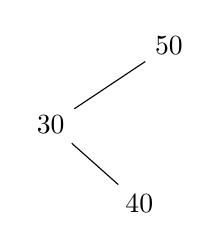
\begin{tikzpicture}[level distance=1.cm,
    level 1/.style={sibling distance=3cm},
  level 2/.style={sibling distance=2.25cm},
  level 3/.style={sibling distance=1.125cm},
  level 3/.style={sibling distance=1.12cm},
  ]
\node{50} child  {node{30} child  [missing]
child  {node{40} }
}
child  [missing]
;

\end{tikzpicture}\caption{}\label{t3}
  \end{subfigure}
  \begin{subfigure}{.225\textwidth}
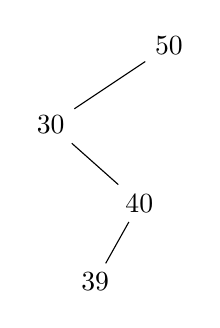
\begin{tikzpicture}[level distance=1.cm,
    level 1/.style={sibling distance=3cm},
  level 2/.style={sibling distance=2.25cm},
  level 3/.style={sibling distance=1.125cm},
  level 3/.style={sibling distance=1.12cm},
  ]
\node{50} child  {node{30} child  [missing]
child  {node{40} child  {node{39} }
child  [missing]
}
}
child  [missing]
;

\end{tikzpicture}\caption{}\label{t4}
\end{subfigure}
\begin{subfigure}{.225\textwidth}
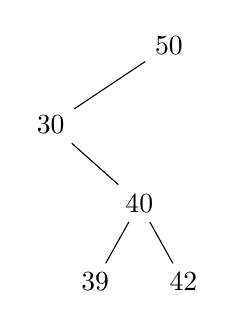
\begin{tikzpicture}[level distance=1.cm,
    level 1/.style={sibling distance=3cm},
  level 2/.style={sibling distance=2.25cm},
  level 3/.style={sibling distance=1.125cm},
  level 3/.style={sibling distance=1.12cm},
  ]
\node{50} child  {node{30} child  [missing]
child  {node{40} child  {node{39} }
child  {node{42} }
}
}
child  [missing]
;

\end{tikzpicture}\caption{}\label{t5}
\end{subfigure}
\begin{subfigure}{.225\textwidth}
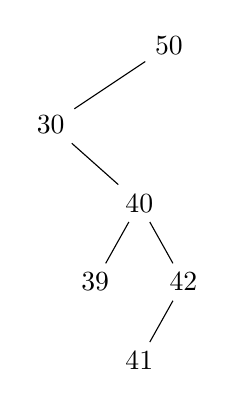
\begin{tikzpicture}[level distance=1.cm,
    level 1/.style={sibling distance=3cm},
  level 2/.style={sibling distance=2.25cm},
  level 3/.style={sibling distance=1.125cm},
  level 3/.style={sibling distance=1.12cm},
  ]
\node{50} child  {node{30} child  [missing]
child  {node{40} child  {node{39} }
child  {node{42} child  {node{41} }
child  [missing]
}
}
}
child  [missing]
;

\end{tikzpicture}\caption{}\label{t6}
\end{subfigure}
\caption{Insertions successives dans un arbre binaire}\label{ibin}
\end{figure}
\end{center}

Évidemment, dans l'exemple donné ci-dessus on aurait pu remplacer les
nombres par des chaînes de caractères, ou tout type d'objets qu'on
peut comparer entre eux.

Considérons maintenant un arbre binaire de $n$ niveaux ($n =
2,3,...$).

\textbf{ C'est là que ça devient remarquable!}
Pour retrouver un nombre dans l'arbre il faut parcourir au plus $n$
niveaux, soit encore faire $n$ comparaisons et $n$ branchements au
plus.

Mais combien y a-t-il de  n{\oe}uds et donc \emph{objets} (de nombres)
  rangés dans un 
arbre de $n$ niveaux? On suppose que l'arbre est complet (cf. figure
\ref{gcomplet}), c'est à dire que tous les niveaux sont complètement occupés:
\begin{figure}
\begin{tikzpicture}[level distance=1.cm,
    level 1/.style={sibling distance=5cm},
  level 2/.style={sibling distance=2.5cm},
  level 3/.style={sibling distance=1.25cm},
  level 3/.style={sibling distance=1.6cm},
  ]

\node{.} child  {node{.} child  {node{.} }
child  {node{.} }
}
child  {node{.} child  {node{.} }
child  {node{.} }
}
;
\end{tikzpicture}
\caption{arbre binaire complet (3 niveaux)}\label{gcomplet}
\end{figure}

\begin{itemize}
\item au niveau 1: $1$.
\item au niveau 2: $2$, soit en tout $2+1 =3$ dans l'arbre.
\item au niveau 3: $4$ , soit en tout $1+ 2 +4 = 7$ dans l'arbre
\item ...
\item au niveau $n$: il y a $2^{n-1}$ n{\oe}uds, ce qui fait qu'entre
  le niveau 1 et le niveau $n$ (compris), on stocke
  $1 +2 + 2^2 + 3^2+ \ldots+ 2^{n-1}$ soit   exactement $2^n - 1$ n{\oe}uds.
\end{itemize}

La recherche est \emph{très rapide}:
\begin{itemize}
  \item pour $1000$ objets rangés dans un arbre binaire complet, comme
    $2^{10} =1024$, les recherches se termineront en au plus $10$
    étapes. Dans un arbre binaire complet contenant un milliard d'objets,
    comme  $10^9 = 1000^3 < 1024^3 = 2^{10^3} = 2^{30}$, les 
    recherches se termineront en au plus $30$ étapes. 
  \item Supposons que la population mondiale rangée dans un arbre
    binaire complet (par ordre de date de naissance?): comme il y a
    environ 6 milliards d'individus  ($6 \times 10^9$) on trouve qu'il faut
    au maximum 33 étapes pour trouver un individu!\footnote{Le
      résultat est qu'une recherche parmi $n$ objets coûte au maximum
      $\log_2 n$ opérations ($\log_2 2^p$, c'est $p$).}
\end{itemize}
\subsection{Oui, mais...}
Que se passe t-il quand on insère une liste ordonnée? (voir la figure
\ref{ordo}). 
\begin{figure}
\begin{tikzpicture}[level distance=1.cm,
    level 1/.style={sibling distance=3cm},
  level 2/.style={sibling distance=2.25cm},
  level 3/.style={sibling distance=1.125cm},
  level 3/.style={sibling distance=1.12cm},
  ]
\node{1} child  [missing]
child  {node{2} child  [missing]
child  {node{3} child  [missing]
child  {node{4} child  [missing]
child  {node{5} }
}
}
}
;
\end{tikzpicture}
\caption{Insertion d'une liste ordonnée}
\label{ordo}
\end{figure}
On engendre non pas un arbre binaire (toutes les branches gauches sont
vides) mais une liste et la recherche à un coût qui n'est pas celui
qu'on attend!

Cela vient du fait que le l'arbre n'est pas \emph{équilibré} (\emph{balanced}).

\emph{Un arbre binaire est dit équilibré si les niveaux des feuilles
  diffèrent au plus de 1.}

On peut s'arranger pour garder l'arbre équilibré au fur et à mesure
des insertions. Reprenons comme exemple l'insertion de la liste (1, 2,
3, 4, 5). Après l'insertion de (1) et (2) l'arbre est équilibré (deux
branches, une de longueur 1 --la branche droite--, l'autre de longueur 0
--la branche gauche--). Mais à l'insertion de (3), l'arbre n'est plus
équilibré (voir figure \ref{ins1}).
\begin{figure}
  \begin{subfigure}{.225\textwidth}
\begin{tikzpicture}[level distance=1.cm,
    level 1/.style={sibling distance=3cm},
  level 2/.style={sibling distance=2.25cm},
  level 3/.style={sibling distance=1.125cm},
  level 3/.style={sibling distance=1.12cm},
  ]
\node{1} ;

\end{tikzpicture}
\caption{équilibré}
\end{subfigure}
\begin{subfigure}{.225\textwidth}
\begin{tikzpicture}[level distance=1.cm,
    level 1/.style={sibling distance=3cm},
  level 2/.style={sibling distance=2.25cm},
  level 3/.style={sibling distance=1.125cm},
  level 3/.style={sibling distance=1.12cm},
  ]
\node{1} child  [missing]
child  {node{2} }
;
\end{tikzpicture}
\caption{équilibré}
\end{subfigure}
\begin{subfigure}{.225\textwidth}
\begin{tikzpicture}[level distance=1.cm,
    level 1/.style={sibling distance=3cm},
  level 2/.style={sibling distance=2.25cm},
  level 3/.style={sibling distance=1.125cm},
  level 3/.style={sibling distance=1.12cm},
  ]
\node{1} child  [missing]
child  {node{2} child  [missing]
child  {node{3} }
}
;

\end{tikzpicture}
\caption{\textbf{NON équilibré}}
\end{subfigure}
\caption{Insertion successive de 1, 2, 3}\label{ins1}
\end{figure}
Mais on peut rendre l'arbre équilibré par une transformation illustrée
à la figure \ref{ins2}:
\begin{figure}
  \begin{subfigure}{.225\textwidth}
\begin{tikzpicture}[level distance=1.cm,
    level 1/.style={sibling distance=3cm},
  level 2/.style={sibling distance=2.25cm},
  level 3/.style={sibling distance=1.125cm},
  level 3/.style={sibling distance=1.12cm},
  ]
\node{1} child  [missing]
child  {node{2} child  [missing]
child  {node{3} }
}
;
\end{tikzpicture}
\caption{Non équilibré}\label{ins21}
  \end{subfigure}
  \begin{subfigure}{.225\textwidth}
\begin{tikzpicture}[level distance=1.cm,
    level 1/.style={sibling distance=3cm},
  level 2/.style={sibling distance=2.25cm},
  level 3/.style={sibling distance=1.125cm},
  level 3/.style={sibling distance=1.12cm},
  ]
\node{2} child  {node{1} }
child  {node{3} }
;

\end{tikzpicture}
\caption{Équilibré}\label{ins22}
  \end{subfigure}
  \caption{Équilibrage}
  \label{ins2}
\end{figure}
entre \ref{ins21} et \ref{ins22} on a fait remonter (2) d'un niveau,
et du coup (1) vient à sa gauche, et l'arbre binaire est équilibré.

\emph{Ce qui veut dire que, avec cette technique, il est plus rapide de
trouver un objet que dans insérer un.}
